\chapter{Methodology}
% \addcontentsline{toc}{chapter}{Methodology}

This section describes the framework used to investigate the anatomical organization of internal fingerprint ridges through the spatial distribution of sweat duct points acquired from 3D OCT scans. The goal of this methodology is to accurately quantify the spatial distribution of identified sweat duct points to assess the structural continuity and separability of internal ridge geometry. Having this evaluation is important for advancing the development of highly secure and spoof-resistant biometric identification systems that use Level 3 features.

\subsection{Data Acquisition}

High-resolution volumetric OCT data were obtained from fingertip scans using a Spectral Domain OCT system. The finger was positioned on a custom-made mechanical device with a flat glass slide to ensure consistent imaging during scanning. The acquisition parameters for each volumetric scan were controlled to allow detailed 3D reconstructions of the skin surface. Each scan captured a volume of 8 mm in width and 4 mm in depth. The system acquired 800 individual slices with a depth resolution of 0.005 mm. Each B-scan covered 8 mm in length and comprised 1,333 A-scans. The A-scan rate was 20,000 Hz with a sampling rate of 3E+7 Hz and 1,024 samples per A-scan with a frequency of 0.0060 mm. A plate movement of 10 mm UD was also noted.

To begin the analysis of 3D fingerprint structures from OCT data, essential Python libraries were used. Numerical and statistical operations were handled by Numpy and Scipy. For 3D processing of the data, Open3D and PyVista tools were used to complete tasks such as mesh manipulation and point cloud analysis. Sci-kit learning was applied to implement clustering algorithms to group and categorize patterns within the sweat ducts. The captured OCT volumetric data were converted into a polygon (.ply) file format in previous work. These files were loaded into the Open3D library, and high-resolution 3D Poisson surface reconstructed meshes of the SC layer were created (Kazhdan et al., 2006). The sweat duct locations, pre-processed and stored in a Python pickle file, were imported. The ducts were separated into entry points, where they emerge on the internal fingerprint surface, and exit points, where they end on the external fingerprint surface.

\subsection{Filtering and Outlier Removal}

We first focused on understanding the spatial distribution of sweat duct openings by computing the minimum distance between neighboring entry points. We achieved this by constructing a KD-tree, which reduces the computational burden of nearest neighbor searches significantly compared to brute-force methods, especially for large datasets. From these calculations, we measured the distance between each sweat duct and its closest neighbor. This measurement was important for two main reasons:

\begin{enumerate}
    \item It allowed us to identify and remove outliers from the dataset. Sweat ducts that were unusually far from their neighbors were likely to be errors or artifacts and were excluded from further analysis.
    \item It provided insights into the overall organization of the sweat duct network. By examining the distribution of distances, we could infer patterns of connectivity and continuity within the internal ridge structures.
\end{enumerate}
After the completion of these steps, we visualized the 3D fingerprint surface with respective sweat ducts using the interactive scene window in PyVista. Not only did visualizing the fingerprint mesh help as a sanity check for previous calculations, but it also aided in the next step of finding a region of interest (ROI) on the fingerprint.
\subsection{Mesh Cropping and Anatomical Segmentation}

To analyze specific features on a 3D fingerprint mesh, we start by cropping an ROI. Figure~\ref{fig:boundary_box} shows how this is done using an interactive bounding box tool, which allows a user to shape a virtual box around the desired area within the 3D mesh of the SC. The coordinates of the box are saved and used to crop down both the 3D mesh and associated sweat duct points, making this an important step because it isolates only the data relevant to the selected region of ridges and sweat ducts.
\begin{figure}[h!]
    \centering
    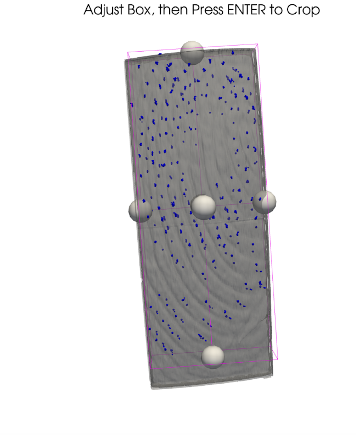
\includegraphics[width=0.5\textwidth]{images/Boundary_Box.png}
    \caption{An interactive bounding box tool used for selecting the ROI on the 3D fingerprint mesh.}
    \label{fig:boundary_box}
\end{figure}

Following the isolation of the cropped mesh and its set of sweat duct points, the next phase involved the segmentation of the dataset using an interactive plane widget. Figure~\ref{fig:cutting_plane} displays how this allows a user to define a cutting plane within the 3D visualization by positioning the plane to divide the cropped mesh and its sweat duct points along its X-axis median. The key benefit of this step is its ability to isolate a specific anatomical section of the internal fingerprint for further computational examination. Once the plane's position and orientation are confirmed, the split is computationally performed by selecting the part of the mesh and points residing beneath the plane. Additionally, any remaining pieces of the SC layer and floating points were identified and removed to give a clear visualization of the internal fingerprint surface. To clean up the high-density regions of sweat duct points, we applied the Density-Based Spatial Clustering of Application with Noise (DBSCAN) algorithm independently to the cluster of sweat duct points \parencite{esterDensityBasedAlgorithmDiscovering}. DBSCAN is a good choice for analyzing anatomical data because it can identify clusters of any shape and is resistant to noise. After clustering, we calculate a centroid for each cluster by averaging the coordinates of all the points within it. This gives us a smaller, more manageable set of representative sweat duct locations for each region.
\begin{figure}[h!]
    \centering
    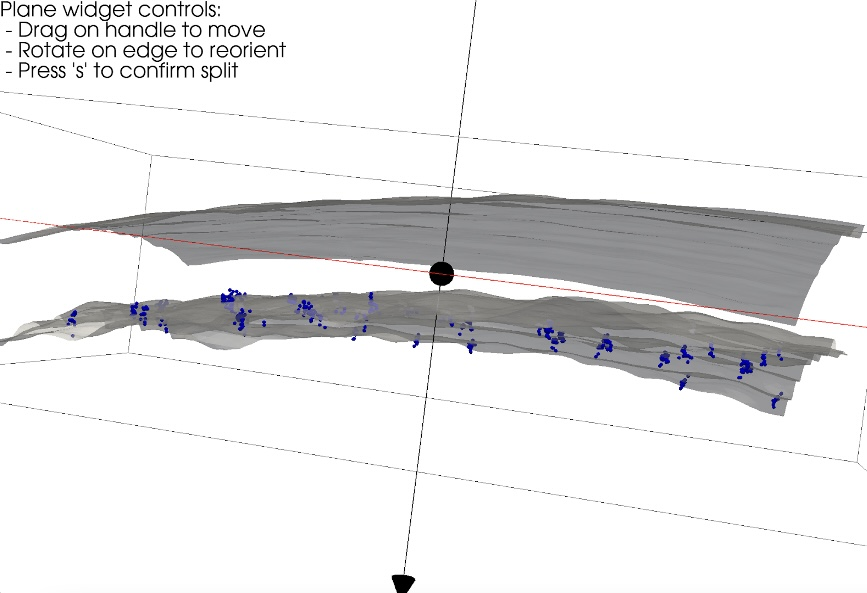
\includegraphics[width=0.8\textwidth]{images/Mesh_Splitting.jpg}
    \caption{An interactive plane widget used to segment the cropped mesh and sweat duct points along the X-axis median.}
    \label{fig:cutting_plane}
\end{figure}
\subsection{Analysis of All Sweat Duct Points}

For a detailed analysis of specific features, we conduct a comprehensive analysis of all identified sweat duct points and their local neighborhoods. The program automatically processes every reduced sweat duct point and its eight nearest neighbors to perform an aggregate, global analysis. This approach provides a broader, more accurate understanding of the internal fingerprint surface. Our analysis performed on the entire set of points consists of three parts: surface curvature, spatial distribution, and normal vector orientation. By performing this comprehensive analysis, we gain insight into the local geometry of the sweat duct points and the internal surface of the fingerprint.

We performed a curvature analysis of the mesh's local curvature to measure how much the surface bends or deviates from a flat plane. We calculated a specific mathematical measure of this bending, known as mean curvature, for each vertex on the mesh. We then extracted the curvature values for all sweat duct points and their nearest neighbors to build a color-coded visualization to display the intensity of the curvature directly on the surface of the mesh. This helps determine if the sweat ducts were located in flatter areas or regions with more curvature. We also conducted a statistical test to determine if the mean curvature of the entire set of points was significantly different from zero, which would suggest the area was not flat. We used a one-sample t-test with the null hypothesis that the region was flat, and also reported the standard deviation of the curvature values to provide a measure of the overall surface complexity.

To understand the spatial arrangement of the sweat ducts, we calculated the pairwise distances between all sweat duct points and their nearest neighbors. We visualized these distances in a heatmap to provide a clear representation of how close or far each point was from the others. Having consistent distances in the heatmap would suggest an organized, uniform pattern, whereas varying distances would indicate a more irregular distribution.

Our final analysis focused on the orientation of the sweat duct points relative to the surface. For each point on the mesh, a normal vector was calculated using surface triangulation. A normal vector is a line perpendicular to the surface at that specific point. We then calculated the dot product between the normal vector of each sweat duct point and the normal vectors of its neighbors. This value quantified the degree of alignment between the vectors. A dot product value close to 1 indicated that the vectors were nearly identically aligned, while lower values suggested a greater difference in orientation. We created a bar chart to visualize the distribution of all alignment scores. Also, we performed a one-sample t-test to determine whether the average orientation of the neighboring points was significantly different from a state of perfect alignment, such as a dot product of 1. This analysis helped us understand if the sweat ducts tended to emerge on relatively flat or uniformly sloped areas of the fingerprint.